\section{Versuchsaufbau/-durchführung}
\subsection{Justage}
Zunächst ist es erforderlich die beiden Schwingkreise auf die selbe Resonanzfrequenz einzustellen.
Hierzu wird der Aufbau gemäß Abbildung \ref{fig: resonanzfrequenz} verwendet, der je einmal
für beide Schwingkreise aufgebaut wird. Die Werte der verwendeten Bauteile lauten:
\begin{align}
  L &= \SI{23.954}{\milli\henry} \\
  C &= \SI{0.7932}{\nano\farad}.
  \label{eq: bauteile}
\end{align}
Im Falle der Resonanz beträgt die Phasendifferenz zwischen Generatorspannung und Schwingkreisstrom $\frac{\pi}{2}$.
Die Lissajou-Figur entspricht hier also einem Kreis.
Die variable Kapazität des zweiten Schwingkreises wird so eingestellt, dass
die Resonanzfrequenzen übereinstimmen.
\begin{figure}
  \centering
  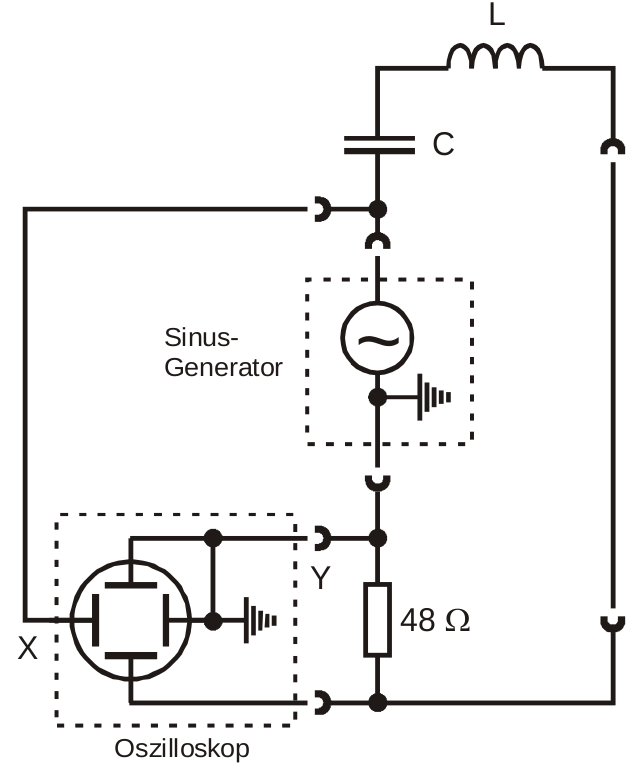
\includegraphics[width = 5cm]{pics/aufbau_resonanzfrequenz.png}
  \caption{Aufbau zur Bestimmung der Resonanzfrequenz \cite{anleitung355}}
  \label{fig: resonanzfrequenz}
\end{figure}

\subsection{Untersuchung der Schwebungen}
Unter variablem Kopplungskondensator $C\ua{k}$ soll das Verhältnis zwischen Schwebungs- und Schwingungsfrequenz ermittelt werden.
Hierzu wird der Aufbau gemäß Abbildung \ref{fig: schwebung} genutzt. Im linken Schwingkreis wird dabei eine Rechteck-Spannung
angelegt. Auf dem Oszilloskop wird die Anzahl Schwingungsmaxima innerhalb eines Schwebungsbauches abgezählt.

\begin{figure}
  \centering
  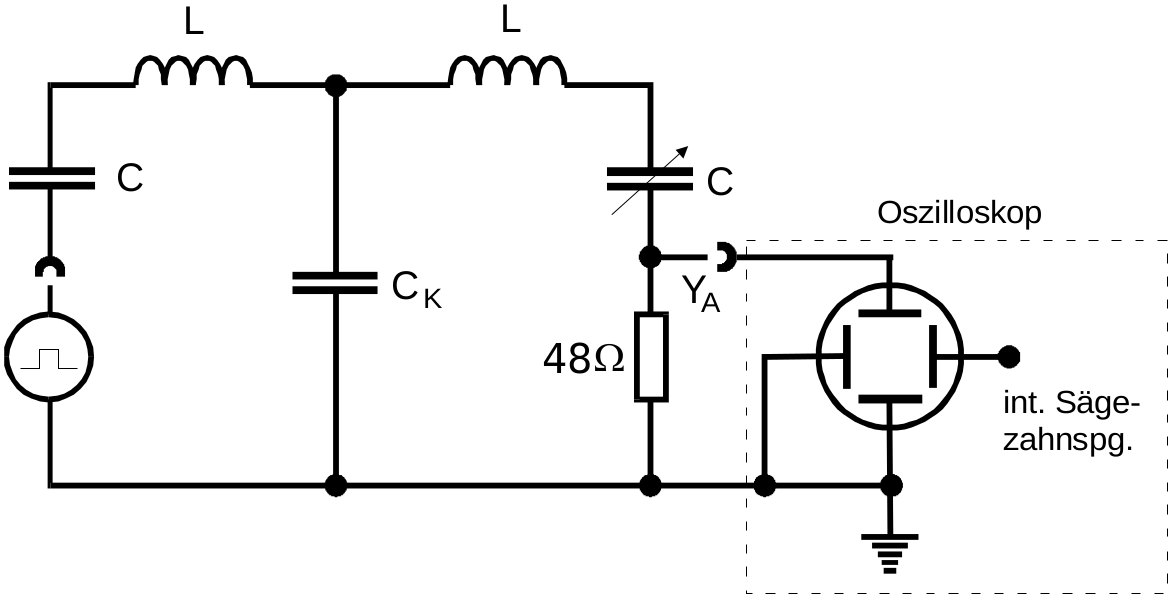
\includegraphics[width = 10cm]{pics/aufbau_schwebung.png}
  \caption{Aufbau zur Untersuchung der Schwebungsvorgänge \cite{anleitung355} (bearbeitet)}
  \label{fig: schwebung}
\end{figure}

\subsection{Messung der Fundamentalschwingungen}
Die experimentelle Bestimmung der Größen $\nu_+$ und $\nu_-$ soll durch zwei verschiedene Methoden geschehen. Zunächst wird der Aufbau \ref{fig: schwebung}
geringfügig modifiziert. Die Rechteckspannung wird durch eine Sinusspannung ersetzt und auf den X-Eingang des Oszilloskops gelegt, welches auf die X-Y-Option
eingestellt wird. Die Phase zwischen der Generatorspannung und der abfallenden Spannung am $\SI{48}{\ohm}$ Widerstand verschwindet für die Resonanzfrequenzen.
Für variable $C\ua{k}$ werden also mittels der \emph{Measure}-Einstellung des Oszilloskops jene Frequenzen ermittelt, für die sich die Lissajou-Figur als Gerade darstellt.\par %Ein Übergang schreiben
Nun zur zweiten Methode. Wie in der Theorie erwähnt, erreicht der Strom $I_2$ und damit auch die über den Widerstand abfallende Spannung zwei Maxima für die Fundamentalfrequenzen.
Das Oszilloskop wird auf den Y-T-Betrieb umgeschaltet und der Spannungsverlauf in Abhängigkeit von der Frequenz untersucht. Hierzu wird ein Frequenzsweep
der Periode $\SI{1}{\second}$ verwendet. Aus Anfangs- und Endfrequenz, sowie den mit dem Oszilloskop gemessenen Zeitdistanzen der Maxima zum Anfangspunkt
des Sweeps, können die Fundamentalfrequenzen in der Auswertung berechnet werden.
\newpage
